    \section{Experiments}
    \label{sec:Experiments}
    \subsection{Sử dụng QNN để giải bài toán của mạng nơ ron truyền thống}
    \label{subsec:integration}


    %=============================================================================
    \subsubsection{Bài toán Two-Moon Classification (Triển khai bằng PennyLane)}
    %=============================================================================

    Bài toán Two-Moon là một bài toán phân loại nhị phân kinh điển, trong đó dữ liệu được phân bố theo hai hình bán nguyệt lồng vào nhau. Đây là bài toán phi tuyến tính, đòi hỏi mô hình phải học được ranh giới quyết định phức tạp.

    Dữ liệu được sinh ra bằng hàm \texttt{make\_moons} từ thư viện scikit-learn với các cấu hình sau:

    \begin{table}[H]
    \centering
    \caption{Cấu hình thí nghiệm cho bộ dữ liệu Two-Moon}
    \label{tab:dataset_config}
    \begin{tabular}{ll}
    \toprule
    \textbf{Tham số} & \textbf{Giá trị} \\
    \midrule
    Sample sizes & 1,000 và 10,000 \\
    Noise levels & 0.1, 0.5, 0.9 \\
    Train/Validation & 75\% / 25\% \\
    Random seed & 42 \\
    \bottomrule
    \end{tabular}
    \end{table}

    Mỗi lớp (Class 0 và Class 1) có số lượng mẫu cân bằng (50\% mỗi lớp). Hình \ref{fig:dataset_distribution} minh họa phân bố dữ liệu với các mức nhiễu khác nhau.

    \begin{figure}[H]
    \centering
    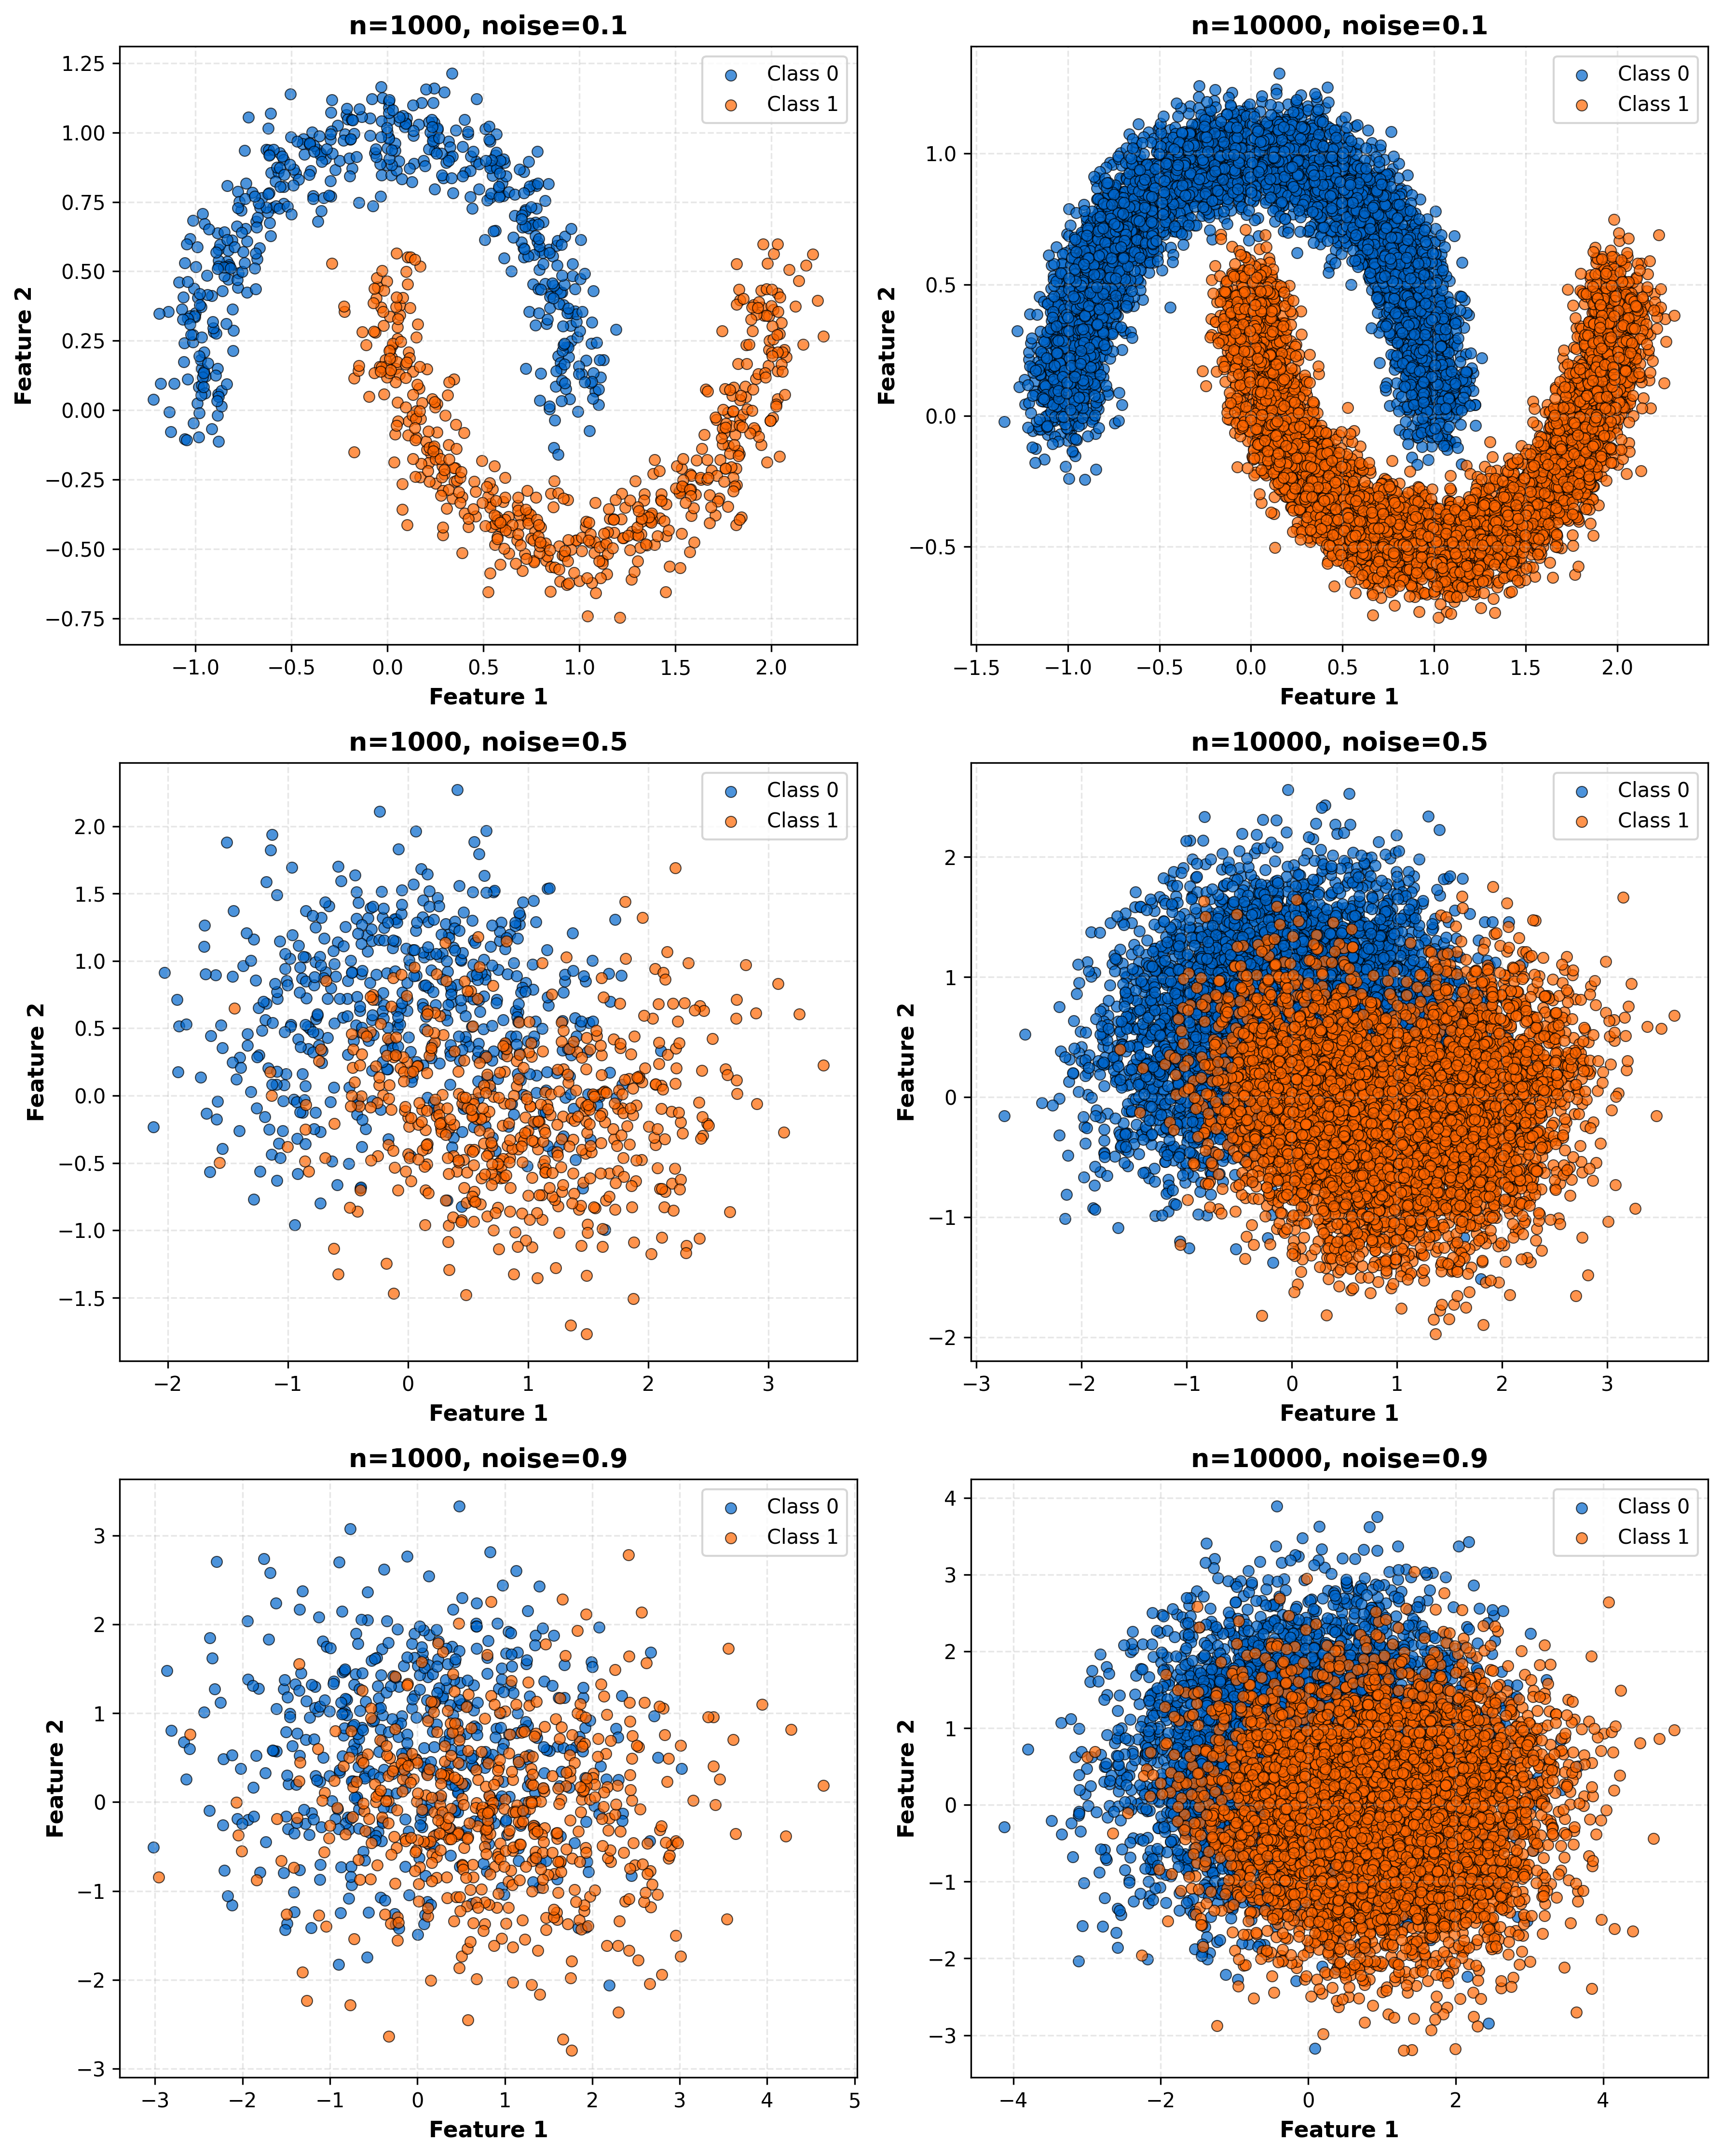
\includegraphics[width=\textwidth]{figures/dataset_distribution.png}
    \caption{Phân bố dữ liệu Two-Moon với các kích thước mẫu (n=1000, n=10000) và mức nhiễu khác nhau (noise=0.1, 0.5, 0.9). Khi mức nhiễu tăng, ranh giới giữa hai lớp trở nên mờ hơn, làm tăng độ khó của bài toán phân loại.}
    \label{fig:dataset_distribution}
    \end{figure}

    \begin{figure}[H]
    \centering
    \includegraphics[width=0.85\textwidth]{figures/gaussian_analysis_n1000.png}
    \caption{Phân tích phân phối Gaussian của các đặc trưng với n=1000 với 3 mức noise khác nhau.}
    \label{fig:gaussian_analysis_n100}
    \end{figure}

    \begin{figure}[H]
    \centering
    \includegraphics[width=0.85\textwidth]{figures/gaussian_analysis_n10000.png}
    \caption{Phân tích phân phối Gaussian của các đặc trưng với n=10000 với 3 mức noise khác nhau.}
    \label{fig:gaussian_analysis_n1000}
    \end{figure}

    \paragraph{Pipeline hoàn chỉnh của QNN}

    \begin{enumerate}
        \item \textbf{Input Layer:} Biến đổi tuyến tính và chuẩn hóa
        \begin{equation*}
            \mathbf{x}' = \tanh(W_{in} \cdot \mathbf{x} + \mathbf{b}_{in}) \cdot \pi
        \end{equation*}
        
        \item \textbf{Angle Embedding:} Mã hóa vào trạng thái lượng tử
        \begin{equation*}
            |\psi(\mathbf{x}')\rangle = \bigotimes_{i=0}^{n-1} R_Y(x'_i)|0\rangle
        \end{equation*}
        
        \item \textbf{Variational Circuit:} $L$ layers với cấu trúc rotation + entanglement
        \begin{equation*}
            U(\boldsymbol{\theta}) = \prod_{l=1}^{L} \left[ \text{CNOT}_{ring} \circ \left(\bigotimes_{i=0}^{n-1} R_Y(\theta_{l,i})\right) \right]
        \end{equation*}
        với $\text{CNOT}_{ring}$: $(i \to i+1 \mod n)$ cho $i = 0, ..., n-1$
        
        \item \textbf{Measurement:} Giá trị kỳ vọng của Pauli-Z
        \begin{equation*}
            z_i = \langle \psi | Z_i | \psi \rangle
        \end{equation*}
        
        \item \textbf{Output Layer:} Biến đổi thành logits
        \begin{equation*}
            \mathbf{y} = W_{out} \cdot \mathbf{z} + \mathbf{b}_{out}
        \end{equation*}
    \end{enumerate}

    \paragraph{Khám phá kiến trúc lượng tử tối ưu}
    ~\\
    \begin{table}[H]
    \centering
    \caption{Kết quả khám phá kiến trúc Quantum với 1000 mẫu, noise=0.1}
    \label{tab:quantum_arch}
    \begin{tabular}{ccccc}
    \toprule
    \textbf{Cấu hình} & \textbf{Số Qubits} & \textbf{Số Layers} & \textbf{Accuracy} & \textbf{Training Time} \\
    \midrule
    Q2L2 & 2 & 2 & 0.9460 & 21.73s \\
    Q2L4 & 2 & 4 & 0.8770 & 28.11s \\
    Q2L6 & 2 & 6 & 0.9790 & 36.04s \\
    Q3L2 & 3 & 2 & 0.9830 & 29.55s \\
    Q3L4 & 3 & 4 & \textbf{0.9910} & 42.32s \\
    Q3L6 & 3 & 6 & 0.9850 & 56.51s \\
    \bottomrule
    \end{tabular}
    \end{table}

    \begin{itemize}
        \item \textbf{Cấu hình tối ưu:} Q3L4 (3 qubits, 4 layers) đạt accuracy cao nhất 99.10\%.
        
        \item \textbf{Với 2 qubits:} Q2L2 đạt 94.60\% - là lựa chọn hợp lý vì dữ liệu chỉ có 2 features đầu vào, mapping trực tiếp sang 2 qubits. 
        
        \item \textbf{Trade-off:} Tăng số qubits/layers giúp tăng expressibility nhưng cũng tăng thời gian huấn luyện (Q3L6: 57s vs Q2L2: 21s) và nguy cơ overfitting.
    \end{itemize}

    %=============================================================================
    \paragraph{Cấu hình huấn luyện}
    %=============================================================================
    ~\\

    \begin{table}[H]
    \centering
    \caption{Các hyperparameter cho quá trình huấn luyện}
    \label{tab:training_config}
    \begin{tabular}{lc}
    \toprule
    \textbf{Hyperparameter} & \textbf{Giá trị} \\
    \midrule
    Số epochs & 10 \\
    Batch size & 5 \\
    Learning rate & 0.05 \\
    Optimizer & Adam \\
    Loss function & Cross-Entropy \\
    Train/Val split & 75\%/25\% \\
    \bottomrule
    \end{tabular}
    \end{table}

    %=============================================================================
    \paragraph{So sánh kết quả thực nghiệm}
    %=============================================================================
    ~\\
    \begin{table}[H]
    \centering
    \caption{So sánh accuracy và thời gian chạy các mô hình theo số lượng mẫu và mức độ noise}
    \label{tab:results_combined}
    \resizebox{\textwidth}{!}{%
    \begin{tabular}{lccccccccccccc}
    \toprule
    \textbf{Model} & \multicolumn{4}{c}{\textbf{noise=0.1}} & \multicolumn{4}{c}{\textbf{noise=0.5}} & \multicolumn{4}{c}{\textbf{noise=0.9}} \\
    \cmidrule(lr){2-5} \cmidrule(lr){6-9} \cmidrule(lr){10-13}
    & \multicolumn{2}{c}{n=1,000} & \multicolumn{2}{c}{n=10,000} & \multicolumn{2}{c}{n=1,000} & \multicolumn{2}{c}{n=10,000} & \multicolumn{2}{c}{n=1,000} & \multicolumn{2}{c}{n=10,000} \\
    \cmidrule(lr){2-3} \cmidrule(lr){4-5} \cmidrule(lr){6-7} \cmidrule(lr){8-9} \cmidrule(lr){10-11} \cmidrule(lr){12-13}
    & Acc & Time & Acc & Time & Acc & Time & Acc & Time & Acc & Time & Acc & Time \\
    \midrule
    Random Forest & \textbf{0.9980} & 8.72 & 0.9978 & 85.78 & 0.8050 & 9.35 & \textbf{0.8215} & 90.53 & 0.7260 & 8.86 & 0.7233 & 93.59 \\
    Classical NN & 0.9960 & 2.21 & 0.9925 & 21.54 & 0.8060 & 2.22 & 0.8174 & 22.11 & 0.5000 & 2.51 & \textbf{0.7264} & 23.61 \\
    Decision Tree & 0.9710 & 2.26 & 0.9857 & 21.71 & 0.7960 & 2.25 & 0.8135 & 25.15 & 0.7000 & 2.39 & 0.7243 & 24.05 \\
    AdaBoost & 0.9950 & 8.72 & 0.9968 & 84.74 & \textbf{0.8100} & 9.18 & 0.8214 & 88.79 & \textbf{0.7280} & 8.90 & 0.7214 & 94.77 \\
    SVM & 0.9950 & 1.85 & 0.9980 & 17.37 & 0.8060 & 1.84 & 0.8197 & 18.35 & 0.7010 & 1.91 & 0.7153 & 18.92 \\
    Naive Bayes & 0.9940 & 1.78 & 0.9981 & 16.98 & 0.7870 & 2.06 & 0.8092 & 18.55 & 0.7010 & 1.74 & 0.7175 & 18.63 \\
    Logistic Reg. & 0.8700 & 1.27 & 0.8833 & 12.40 & 0.7970 & 1.28 & 0.8063 & 12.99 & 0.7210 & 1.34 & 0.7119 & 13.59 \\
    Quantum NN & 0.9430 & 41.98 & \textbf{0.9982} & 410.69 & 0.7950 & 43.88 & 0.8034 & 438.35 & 0.7010 & 43.10 & 0.6940 & 424.81 \\
    \bottomrule
    \end{tabular}%
    }
    \end{table}


    %=============================================================================
    \paragraph{Phân tích thời gian huấn luyện Quantum NN}
    %=============================================================================
    ~\\
    \begin{table}[H]
    \centering
    \caption{Chi tiết thời gian huấn luyện Quantum NN}
    \label{tab:qnn_time}
    \begin{tabular}{cccccc}
    \toprule
    \textbf{n\_samples} & \textbf{noise} & \textbf{Encoding} & \textbf{Pure Training} & \textbf{Inference} & \textbf{Total} \\
    \midrule
    1,000 & 0.1 & 0.230s (0.5\%) & 41.73s (99.5\%) & 0.019s & 41.98s \\
    1,000 & 0.5 & 0.143s (0.3\%) & 43.72s (99.7\%) & 0.014s & 43.88s \\
    1,000 & 0.9 & 0.258s (0.6\%) & 42.82s (99.4\%) & 0.023s & 43.11s \\
    \midrule
    10,000 & 0.1 & 0.325s (0.1\%) & 410.33s (99.9\%) & 0.034s & 410.69s \\
    10,000 & 0.5 & 0.391s (0.1\%) & 437.92s (99.9\%) & 0.035s & 438.35s \\
    10,000 & 0.9 & 0.489s (0.1\%) & 424.27s (99.9\%) & 0.047s & 424.81s \\
    \bottomrule
    \end{tabular}
    \end{table}

    \begin{figure}[H]
    \centering
    \includegraphics[width=\textwidth]{figures/training_time_comparison.png}
    \caption{So sánh thời gian huấn luyện giữa các mô hình. Quantum NN yêu cầu thời gian huấn luyện lớn hơn đáng kể so với các mô hình cổ điển do chi phí tính toán của mạch lượng tử.}
    \label{fig:training_time}
    \end{figure}

    \textbf{Nhận xét:}
    \begin{itemize}
        \item \textbf{Bottleneck chính:} Phần lớn thời gian huấn luyện (>99\%) là do quá trình tính gradient và cập nhật tham số (Pure Training), trong khi thời gian mã hóa dữ liệu (Encoding) và inference chiếm tỷ lệ rất nhỏ (<1\%).
        
        \item \textbf{Scalability:} Khi tăng từ n=1,000 lên n=10,000 (10x), thời gian huấn luyện QNN tăng khoảng 10x (từ $\sim$42-44s lên $\sim$410-438s), cho thấy độ phức tạp tuyến tính $O(n)$ theo số lượng mẫu.
        
        \item \textbf{So sánh với mô hình cổ điển:} QNN chậm hơn các mô hình thông thường. Tuy nhiên, các mô hình như Random Forest và AdaBoost cũng có thời gian huấn luyện chậm do có cơ chế ensemble.
        
        \item \textbf{Ảnh hưởng của noise:} Mức noise không ảnh hưởng đáng kể đến thời gian huấn luyện, cho thấy chi phí tính toán chủ yếu phụ thuộc vào kích thước dữ liệu và kiến trúc mạch.
    \end{itemize}

    % %=============================================================================
    % \paragraph{Đường cong học tập (Learning Curves)}
    % %=============================================================================

    % \begin{figure}[H]
    % \centering
    % \includegraphics[width=\textwidth]{figures/learning_curves_n1000.png}
    % \caption{Đường cong học tập của các mô hình với n=100. Mỗi hàng hiển thị một mô hình, mỗi cột hiển thị Loss và Accuracy cho Training và Validation ứng với 3 mức noise khác nhau (0.05, 0.1, 0.2).}
    % \label{fig:learning_curves_n100}
    % \end{figure}

    % \begin{figure}[H]
    % \centering
    % \includegraphics[width=\textwidth]{figures/learning_curves_n10000.png}
    % \caption{Đường cong học tập của các mô hình với n=1000. Mỗi hàng hiển thị một mô hình, mỗi cột hiển thị Loss và Accuracy cho Training và Validation ứng với 3 mức noise khác nhau (0.05, 0.1, 0.2).}
    % \label{fig:learning_curves_n1000}
    % \end{figure}
    %=============================================================================
    \paragraph{Ranh giới quyết định (Decision Boundaries)}
    %=============================================================================
    ~\\
    \begin{figure}[H]
    \centering
    \includegraphics[width=\textwidth]{figures/decision_boundaries.png}
    \caption{Ranh giới quyết định của các mô hình trên tất cả các cấu hình. Quantum NN tạo ra ranh giới quyết định mượt mà và có khả năng khái quát hóa tốt, đặc biệt với dữ liệu nhiễu thấp.}
    \label{fig:decision_boundaries}
    \end{figure}

    \subsubsection{Bài toán XOR}


    % %=============================================================================
    % \subsection{Thảo luận và Kết luận}
    % %=============================================================================

    % \paragraph{Ưu điểm của Quantum Neural Network:}
    % \begin{itemize}
    %     \item \textbf{Hiệu suất cao với dữ liệu lớn và nhiễu thấp:} Với n=10,000 và noise=0.1, QNN đạt accuracy cao nhất (99.82\%), vượt trội so với tất cả các mô hình cổ điển bao gồm SVM (99.80\%) và Naive Bayes (99.81\%).
        
    %     \item \textbf{Số tham số compact:} Với cấu hình Q3L4, QNN chỉ cần $3 \times 4 = 12$ tham số cho quantum layer, cộng thêm các tham số từ input/output layers ($2 \times 3 + 3 + 3 \times 2 + 2 = 17$ tham số), tổng cộng khoảng 29 tham số - ít hơn đáng kể so với các mô hình ensemble như Random Forest.
        
    %     \item \textbf{Ranh giới quyết định mượt mà:} QNN tạo ra decision boundary mượt và có khả năng generalization tốt, tránh được hiện tượng overfitting cục bộ như Decision Tree.
    % \end{itemize}

    % \paragraph{Hạn chế:}
    % \begin{itemize}
    %     \item \textbf{Thời gian huấn luyện dài:} QNN yêu cầu thời gian huấn luyện lớn hơn khoảng 19 lần so với Classical NN (410s vs 21s với n=10,000). Đây là bottleneck chính cho việc ứng dụng thực tế.
        
    %     \item \textbf{Hiệu suất kém với nhiễu cao:} Với noise=0.9, QNN đạt accuracy thấp hơn các mô hình cổ điển (69.40\% vs Classical NN 72.64\%), cho thấy quantum circuit nhạy cảm với dữ liệu nhiễu.
        
    %     \item \textbf{Không tối ưu cho dữ liệu nhỏ:} Với n=1,000, các mô hình ensemble như Random Forest (99.80\%) và AdaBoost (99.50\%) cho kết quả tốt hơn QNN (94.30\%).
    % \end{itemize}

    % \paragraph{Kết luận:}
    % Quantum Neural Network thể hiện tiềm năng vượt trội trong các bài toán với:
    % \begin{enumerate}
    %     \item Dữ liệu có kích thước lớn ($n \geq 10,000$)
    %     \item Mức nhiễu thấp (noise $\leq 0.1$)
    %     \item Yêu cầu mô hình compact với ít tham số
    % \end{enumerate}

    % Tuy nhiên, chi phí tính toán cao (do mô phỏng quantum trên máy cổ điển) vẫn là rào cản chính. Với sự phát triển của phần cứng quantum thực tế, những hạn chế này được kỳ vọng sẽ được giải quyết trong tương lai.

    % \begin{table}[H]
    % \centering
    % \caption{Tóm tắt: Mô hình tốt nhất cho từng cấu hình}
    % \label{tab:best_models_summary}
    % \begin{tabular}{cclc}
    % \toprule
    % \textbf{n\_samples} & \textbf{noise} & \textbf{Best Model} & \textbf{Accuracy} \\
    % \midrule
    % 1,000 & 0.1 & Random Forest & 0.9980 \\
    % 1,000 & 0.5 & AdaBoost & 0.8100 \\
    % 1,000 & 0.9 & AdaBoost & 0.7280 \\
    % 10,000 & 0.1 & \textbf{Quantum NN} & \textbf{0.9982} \\
    % 10,000 & 0.5 & Random Forest & 0.8215 \\
    % 10,000 & 0.9 & Classical NN & 0.7264 \\
    % \bottomrule
    % \end{tabular}
    % \end{table}
